\documentclass[14pt]{extreport}
\usepackage{gost}

\begin{document}
\pagestyle{empty} %  выключаем нумерацию
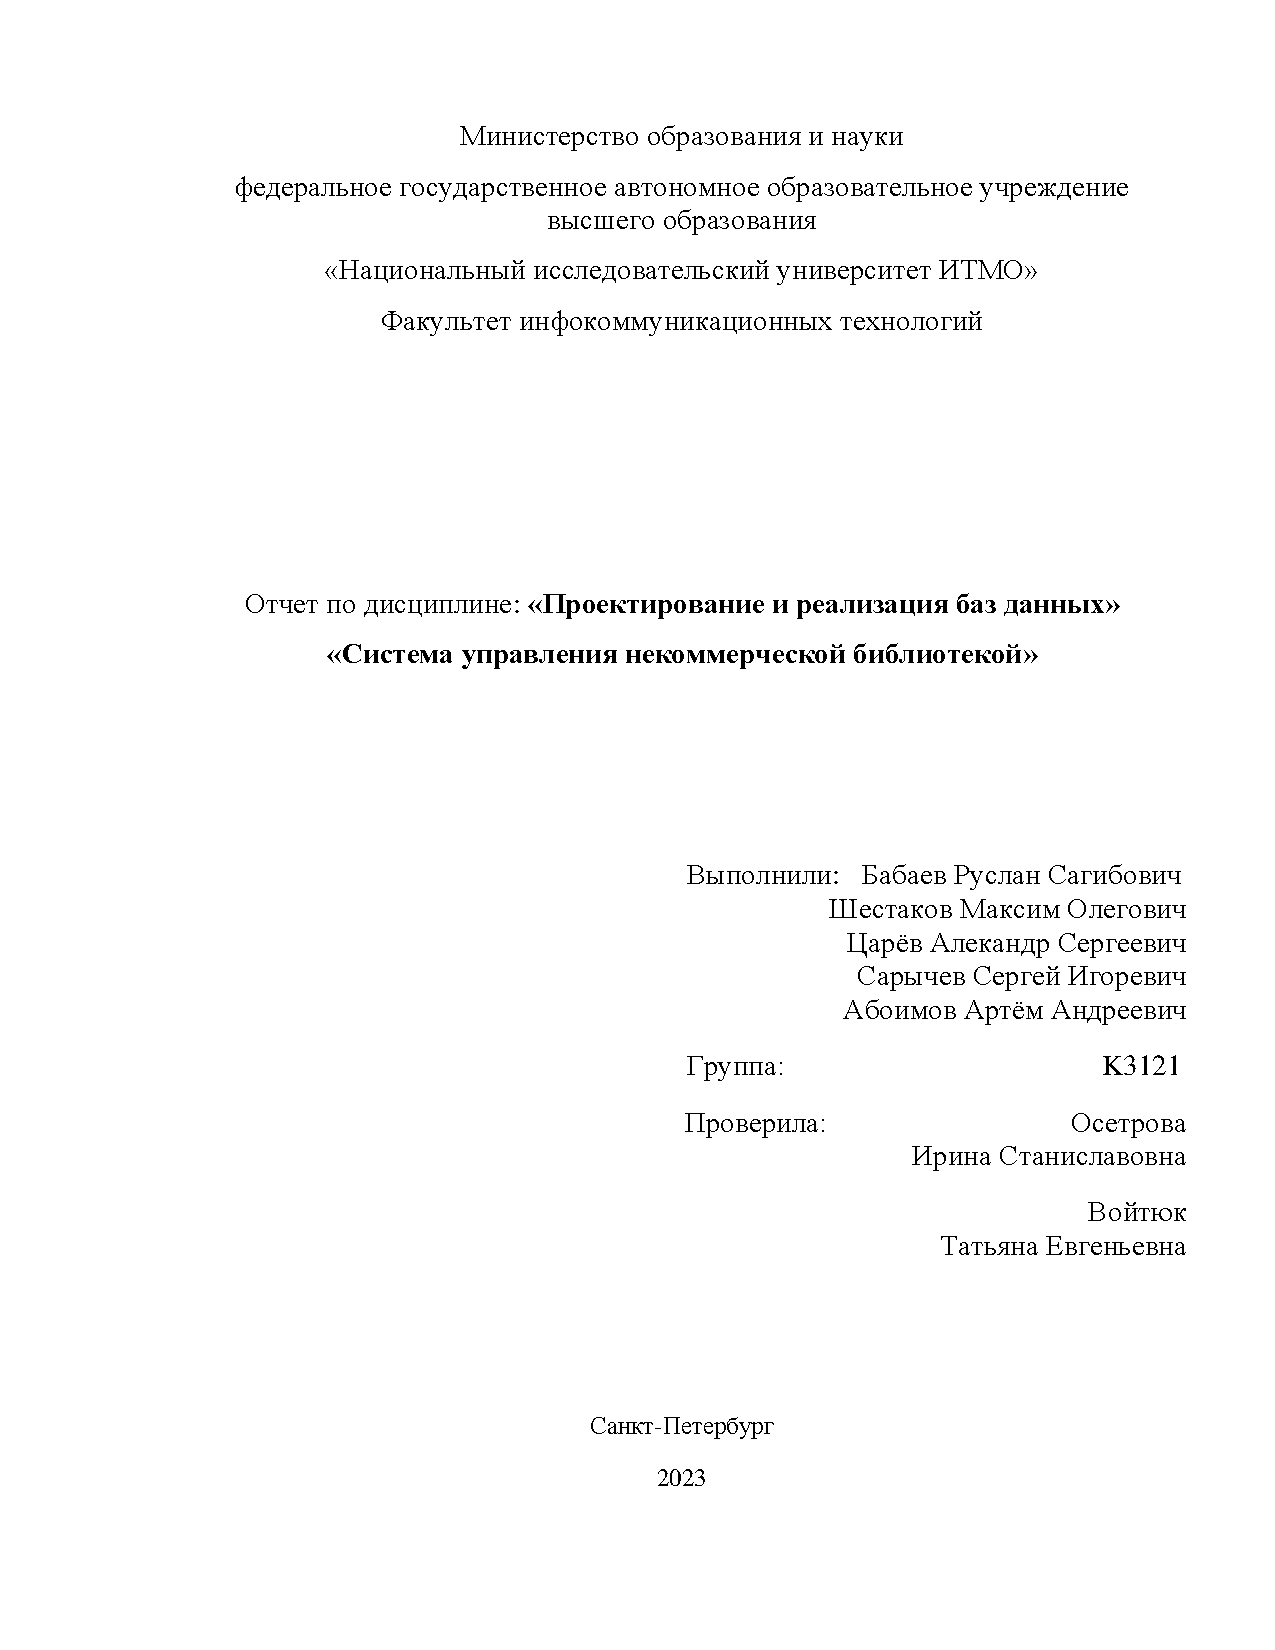
\includepdf[pages=-,pagecommand={}]{title.pdf}

\pagestyle{plain} % включаем нумерацию
\tableofcontents

\intro

\chapter{}

\chapter{}

\chapter{}

\chapter{}

\conclusions

\begin{thebibliography}{2}

\bibitem{bib1} ГОСТ 34.602-89. Информационная технология. Комплекс стандартов на автоматизированные системы. Техническое задание на создание автоматизированной системы.

\bibitem{bib2} Wikipedia [Электронный ресурс]: [сайт]. - URL: \url{https://goo.su/84Cou} (дата обращения 12.12.2022). - Загл. с экрана. - Яз.рус.111

\bibitem{bib3} Figma [Электронный ресурс]: [сайт]. - URL: \url{https://www.figma.com/} (дата обращения 12.12.2022). - Загл. с экрана. - Яз.англ.

\end{thebibliography}

\end{document}


